\section{Introduction}
\label{section:intro}

\emph{Peer-to-peer (P2P)} networks are self-organizing distributed systems where
participating nodes, called \emph{peers}, act as both resource providers and
resource consumers, in contrast to the traditional \emph{client-server} model
where nodes take on the role of pure servers or pure clients. Peer-to-peer
networks have enjoyed immense attention from Internet users, companies, and
researchers and have been widely deployed for over a decade, primarily because
of the great number of features they offer distributed applications that are
built on top of them. These features include:  high availability and robustness,
load-balancing, quality of service, scalability, decentralized administration,
and anonymity. 

Two ``killer'' applications of the peer-to-peer paradigm are, but not limited
to, file-sharing and telephony. P2P file-sharing was originally introduced by
Napster (see Section~\ref{section:background}), which by 2001 was widely
acknowledged as the ``fastest growing Internet application ever" with 26 million
users sharing 80 million songs at the height of its popularity. Other similar
applications quickly followed suit including Gnutella and its descendant,
Limewire, enjoying 3 million concurrently connected peers by the end of 2006
and BitTorrent, connecting over 150 million users. P2P telephony has seen
explosive growth with the advent of Skype. Since its introduction in 2003,
Skype has become extremely popular with more than 650 million users in 2011
\cite{skypetotalusers} and 35 million skypers concurrently online on the 5th of
March 2012 \cite{skypesymusers}.

In addition to file-sharing and telephony, a large number of diverse
applications have been built on top of peer-to-peer systems including:
distributed search engines \cite{yaci}, distributed data storage systems
\cite{kbc_oceanstore_2000,bdet_fsdfs_2000,dkkms_cfs_2001,dr_pastutility_2001,abc_farsite_2002,mmfc_ivy_2002,arla,agebh_dks_2003},
Web caches, archives and publishing systems
\cite{ird_squirrel_2002,bags_youserv_2002,wrc_publius_2000,wm_tangler_2001},
messaging applications \cite{threedegrees}, event notification infrastructures
\cite{rkcd_scribe_2001,cdkr_scribe_2002,agebh_dks_2003}, naming services
\cite{cmm_chorddns_2002}, censor-resistant stores \cite{cswh_freenet_2001} and
lately even cloud-based platforms \cite{mgpj_cloudsnap_2011}.

Peer-to-peer systems are implemented using overlay networks. An \emph{overlay
network} is a virtual system of nodes and logical links, that is built on top of
an existing network intending to provide added value to it (e.g., offering QoS
content distribution over the best effort Internet network). Nodes in the
overlay communicate via virtual connections each of which may correspond to a
path of possibly many physical links in the underlying network.
Figure~\ref{figure:overlay} illustrates a simple four-node overlay constructed
over a wide-area network.

\begin{figure}
\centering
  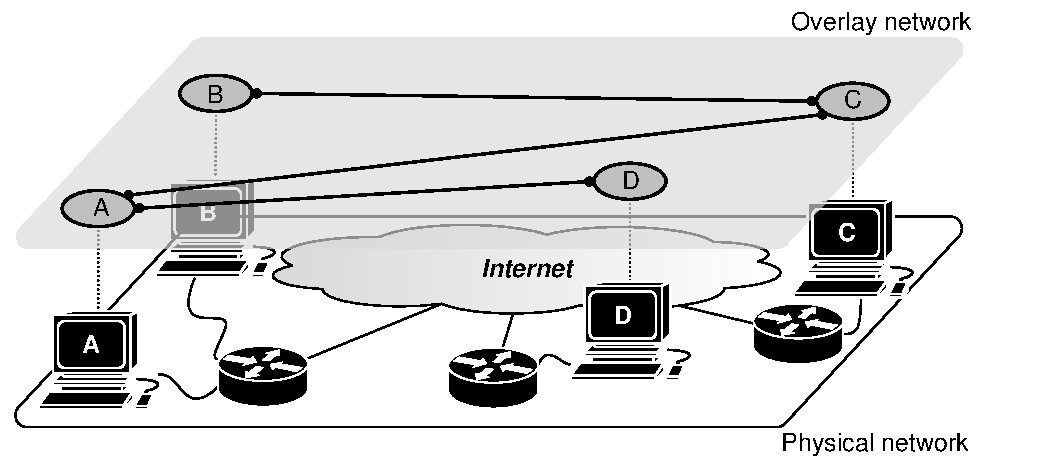
\includegraphics[scale=0.7]{img/pdf/under-over-lay.pdf}
\caption{An example overlay network.}
\label{figure:overlay}
\end{figure}

One of the fundamental issues that defines the efficiency of an overlay network
is how well the overlay maps to the underlying network topology on which it
rests. Consider two nodes\footnote{In the case of peer-to-peer networks,
typically the participating nodes are user PCs sitting at the edge of the
Internet.} that share a link in an overlay network which maps to multiple hops
in the underlying (say IP) topology. If the traffic patterns of the application
are such that traffic flows heavily over the overlay link between the two nodes,
then it is beneficial to construct the overlay topology such that the number of
underlying IP links between these two nodes is minimized.

If the overlay network is constructed such that it does not match the underlying
topology well, the resulting \emph{topology mismatch} (See
Section~\ref{section:background} for a more formal definition) can result in two
significant problems. First, the performance of the application per se, can be
adversely affected since application traffic must flow over a larger,
redundunt, number of physical hops resulting in poor user experience like
extensive search latency or jitter. Second, can cumulatively degrade the
performance of the whole underlying infrastructure, effecting other applications
as well. For example, studies have shown that the extreme popularity of P2P
applications amply deployed everywhere nowadays, result in them contributing the
largest portion of overall Internet traffic
\cite{seroiu_analysiscds_2002,sen_analyzep2ptraffic_2004,krp_ispfear_2005}, with
some reporting that more than 60\% of it, is
P2P-related~\cite{cachelogic,ipoque2007,ipoque2009} and others claiming that it
is expected to reach almost 8 petabytes per month by the end of
2012~\cite{multinteligence}. This is a significant burden for Internet Service
Providers (ISPs) who must handle all this traffic to destination nodes sitting
at the edge of the Internet. If the overlay topology of a peer-to-peer system is
not efficiently constructed, then this burden to the Internet's backbone
infrastructure could be even greater. For example, traffic might have to flow
back and forth several times between two neighboring ISPs as it travels from its
source node in the overlay to its destination node. Thus, it is fundamentally
important that P2P overlay networks are constructed and maintained so that
their topology matches as closely as possible the underlying IP topology. 

For over a decade, several researchers have published profusely on the topology
mismatch problem.  In this paper, we survey this research area and provide a
taxonomy of the proposed solutions. We point out synergies as well as
similarities and differences in the published approaches. Ultimately, our goal
is to help readers sift through the vast amount of literature, to help them
understand the advantages and disadvantages of each of each work, and to provide
them with enough perspective so that when the need arises, they are able to
select amongst the different approaches for their particular application.

The rest of the paper is organized as follows: In
Section~\ref{section:background}, we provide background information on
peer-to-peer overlay architectures including centralized, decentralized
unstructured and decentralized structured peer-to-peer systems. We also formally
define the problem of topology mismatch between an overlay and its underlying
physical network and elaborate on the rationale behind our coarse grained
evaluation of the techniques presented throughout this survey. In
Sections~\ref{section:unstructured} and \ref{section:structured}, we present the
various research efforts for decentralized unstructured and decentralized
structured peer-to-peer systems, respectively. Finally, with
Section~\ref{section:conclusion}, we conclude the paper.
